\section[SGBD orientés colonnes]{SGBD orientés colonnes}
\begin{frame}[allowframebreaks, fragile]{SGBD orientés colonnes}
    \begin{itemize}\itemsep1em
        \item Table Produit: 
        \begin{figure}
            \centering
            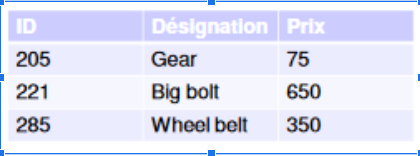
\includegraphics[scale=0.5]{figures/product.PNG}
        \end{figure}
        \item Stockage physique en lignes: 
        \begin{itemize}
            \item[-] 205, Gear, 75;
            \item[-] 221, Big bolt, 650;
            \item[-] 285, Wheel belt, 350;
        \end{itemize}
        \item Stockage physique en colonnes: 
        \begin{itemize}
            \item[-] 205, 221, 285; 
            \item[-] Gear, Big Bolt, Wheel belt;
            \item[-] 75, 650,350;
        \end{itemize}
        \item Recherche par prix:\\
    	\begin{minipage}{0.4\linewidth}
    	   \begin{itemize}
                \item[-] 205, Gear, \textbf{75};
                \item[-] 221, Big bolt, \textbf{650};
                \item[-] 285, Wheel belt, \textbf{350};
           \end{itemize}
    	\end{minipage}
        \begin{minipage}{0.5\linewidth}	
            \begin{itemize}
                \item[-] 205, 221, 285;
                \item[-] Gear, Big Bolt, Wheel belt;
                \item[-] \textbf{75}, \textbf{650}, \textbf{350};
           \end{itemize}
        \end{minipage}
        \item Quelques SGBD orientés colonnes
        \setbeamertemplate{description item}[align left]
        \begin{description}
            \item[Open source :] C-Store, PostgreSQL cstore\_fdw, MariaDB ColumnStore
            \item[Propriétaires :]  DB2, SQL Server, Oracle (in memory), SAP Hana, Teradata, Vertica
            \item[Cloud:] Amazon Redshit, Google BigQuery
        \end{description}
    \end{itemize}
\end{frame}